% !TEX root = main.tex
%
%\begin{figure*}[t] 
%	\begin{center}
%		\scalebox{.4}{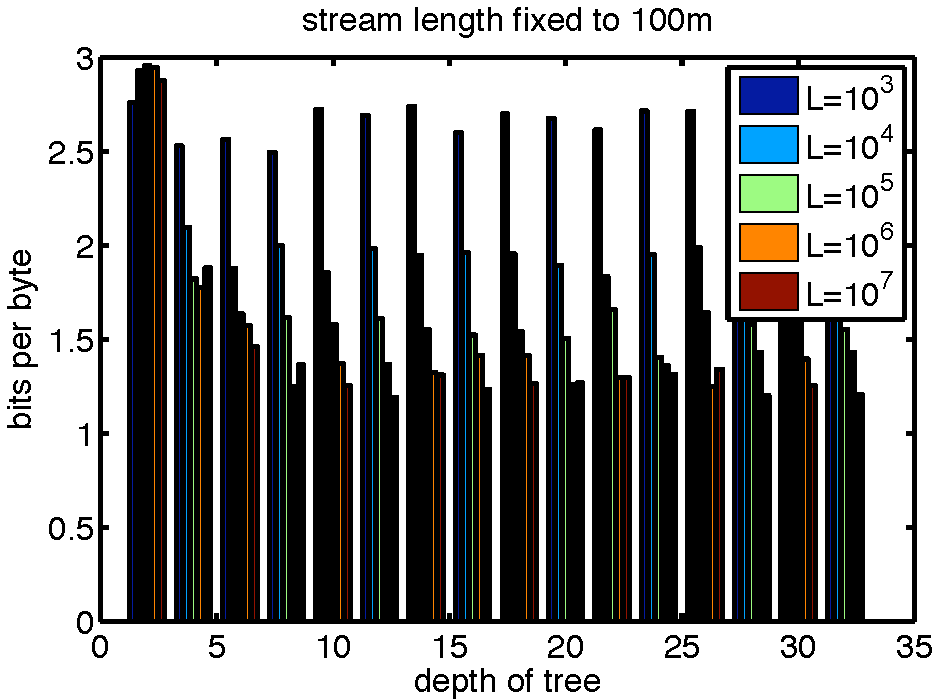
\includegraphics{figs/varying_depths.pdf}} % [clip=true, viewport= 1in 1in 9in 9in]
%		\caption{Average ($\pm$ std.) streaming deplump compression performance as measured in bits in compressed output vs.~bytes in uncompressed input.  Here the depth limit ($D$) and node limit ($L$) are varied.  From this we conclude that setting the depth limit to $D\geq16$ and the node limit to the largest value possible given physical memory constraints leads to optimal compression performance.}
%		\label{fig:varying_depths}
%	\end{center} 
%\end{figure*} 
%
%\begin{figure*}[t] 
%	\begin{center}
%		\scalebox{.6}{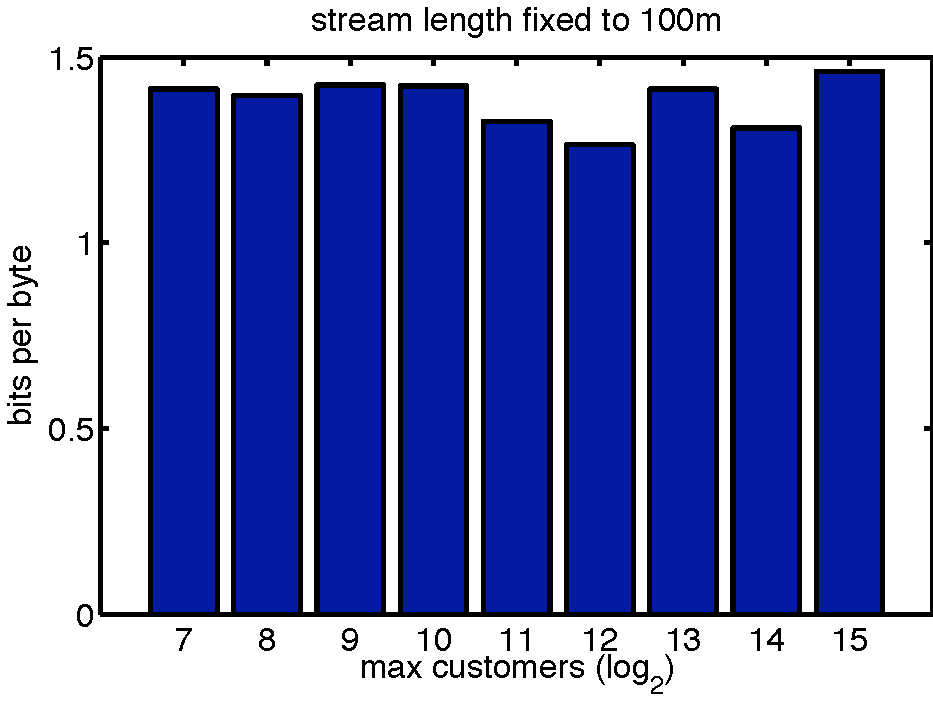
\includegraphics{figs/varying_max_customers.pdf}} % [clip=true, viewport= 1in 1in 9in 9in]
%		\caption{Performance for varying max allowable customers $k$.}
%		\label{fig: varying_max_customers}
%	\end{center} 
%\end{figure*} 
%
\begin{figure*}[t] 
	\begin{center}
		\scalebox{.4}{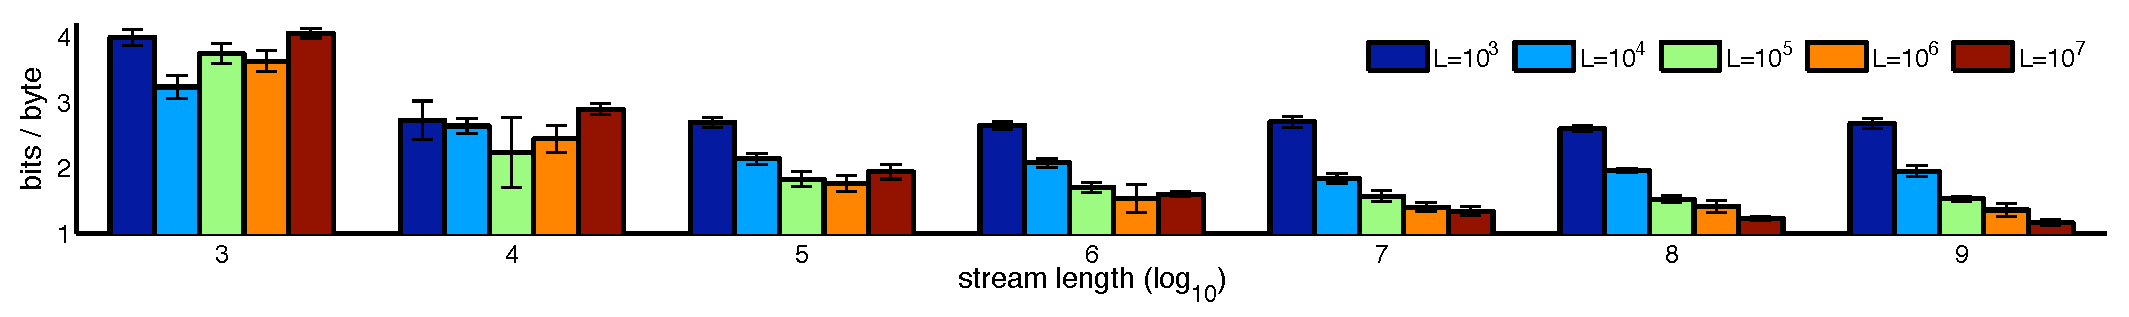
\includegraphics{figs/varying_stream_length.pdf}} % [clip=true, viewport= 1in 1in 9in 9in]
		\caption{Average ($\pm$ std.) SM predictive performance in terms of average number of bits required to encode each byte of uncompressed input.  Here the input stream length and number of distinctly estimated conditional distributions ($L$) are varied.  Observe that average performance monotonically improves as a function of both the input sequence length and of the exactness of the approximation. That performance varies as a function of model complexity for the same size data suggests that the approximate posterior used to compute average model performance may not accurately average over uncertainty about the larger models' parameters. %Also, it can be seen that large node limits may actually hurt compression performance for small input sequences.
		}
		\label{fig:varying_stream_length}
	\end{center} 
\end{figure*} 
%
\section{Experiments}
\label{sec:experiments}

%As the performance of batch deplump was established relative to other lossless compressors for a variety of datatypes in \citep{Gasthaus2010}, we focus our experiments on establishing a) that the approximations to inference in the sequence memoizer combined in this paper in order to make deplump a streaming compressor do not significantly adversely affect compression performance, b) that the resulting compressor can indeed compress extremely long sequences as the asymptotic guarantees would suggest it should, and c) which settings of the approximation parameters produce the best compression performance.
%Most of the experiments included in this paper use a complete Wikipedia text content dump \citep{Wikipedia2010} as a test corpus (26.8Gb uncompressed, 7.8Gb gziped, 3.8Gb paq9a'ed, both with default parameters, and 4.0Gb deplumped).  

%To establish what approximation parameters produce the best compression results we first ran streaming deplump on the first 100Mb section of the corpus limiting the depth to two different values ($D=16$ and $D=1024$) with a fixed limit on the number of nodes in the tree ($L=10^6$).  We observed that in both cases only very few nodes had high total counts ($c > 8,192$) suggesting that it might be possible to set the count upper bound conservatively ($k= 8,192$) without significant compression performance degradation.  %That compression performance should not be affected by a reasonable count bound follows intuitively from the fact that in byte sequences $|\Sigma| = 256$ and setting $k=10,000$ is similar in effect to using 10,000 observations to estimate a 256 element discrete distribution.  
%To ensure that compression performance did in fact not suffer, we compressed ten 100Mb subsections of the corpus (sampled randomly with replacement) for multiple values of $k$ between 128 and 32,768 (fixing $L=10^6$ and $D=16$).  We observed that average compression performance indeed varied insignificantly over all values of $k$.

In order to achieve asymptotically constant storage and linear time cost to generate a single posterior sample, the number  $L$ of conditional distribution estimates maintained, the maximum number $k$ of observations held at each node, the length of a buffer $T$ holding observations  all must be capped.  Optionally the maximum context length $D$ can also be capped.  The resulting approximate SM can be interpreted as a semi-greedy approximation to the full SM in which the number of represented conditional density estimates is constrained to be simultaneously less than both the number of nodes in the suffix tree representation of the ``remembered'' sequence of observations of length $T$ and the hard constraint on the number of conditional distribution estimates $L$.  It can also be interpreted as a dependent nonparametric model \citep{Bartlett2010}.
%
%The interplay between limiting the number of nodes in the tree and restricting the depth of the tree was explored (results for which are shown in Figure~\ref{fig:varying_depths}).  Here $k$ was set to 8,192, while $L$ and the depth of the tree $D$ were varied as indicated in the figure. 
The performance of SM-approximations have been explored by modeling subsections of length $L$ sampled with replacement from the complete Wikipedia text content dump \citep{Wikipedia2010}.  (Figure~\ref{fig:varying_stream_length}).  In these experiment $k=8,192$, $T=10^8$, and $D=16$ while $L$ varied as shown in the figure.   The largest value of $L$ has performance indistinguishable from that of the full sequence memoizer for values of stream length up to $10^7$.  The full sequence memoizer could not be instantiated for the largest datasets so no comparison can be provided. %(, , , , $\mathcal{D} = [.5, .7, .8, .82, .84, .88, .91, .92, .93, .94, .95, .93]$, and $\eta=0.0001$)  
%Figure~\ref{fig:varying_depths} indicates that compression performance becomes essentially indistinguishable for depth restrictions greater than $D=10$.  However, this figure also suggests that compression performance improves as a function of the number of nodes in the tree for depths 6 and greater.  Figure~\ref{fig:varying_stream_length} illustrates that the algorithm not only scales to very long sequences, but average compression performance continues to improve as the sequence grows.  Using a large value of $L$ appears to be beneficial for very long sequences.

%We chose values for the approximating parameters ($D=32$, $L=10^7$, $k=8,192$, $T=10^8$, $\mathcal{D} = [.5, .7, .8, .82, .84, .88, .91, .92, .93, .94, .95, .93]$, and $\eta=0.0001$) and compared streaming deplump to batch deplump.  In this experiment we achieved compression performance of 1.67 bites per byte on the 100Mb Wikipedia corpus excerpt used for the Hutter Prize \citep{Hutter2006} using the streaming variant of deplump.  Batch deplump \citep{Gasthaus2010} achieved 1.66 bits per byte.  If we were to have instead taken the most obvious approach to streaming compression, namely, compressing the sequence in blocks until a memory bound is hit and then starting over, performance falls to 1.88 bits per byte (limiting the sequence length of each block such that the resulting batch deplump compressor used a maximum amount of memory roughly equivalent to the amount of memory used by the streaming variant). These results further demonstrate that the streaming variant of deplump is a significant improvement over the na\"{\i}ve approach to compression of streaming data using batch deplump.

%\begin{figure*}[t] 
%	\begin{center}
%		\scalebox{1}{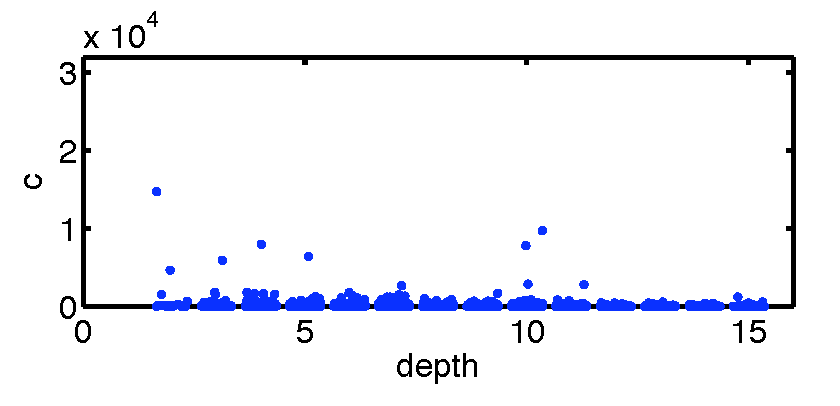
\includegraphics{figs/scatter_16.pdf}} % [clip=true, viewport= 1in 1in 9in 9in]
%		\caption{Scatter plots to explore the relationship between the depth of a node and the total count}
%		\label{fig:restaurant_plots}
%	\end{center} 
%\end{figure*} 

%\begin{figure*}[t] 
%	\begin{center}
%		\scalebox{1}{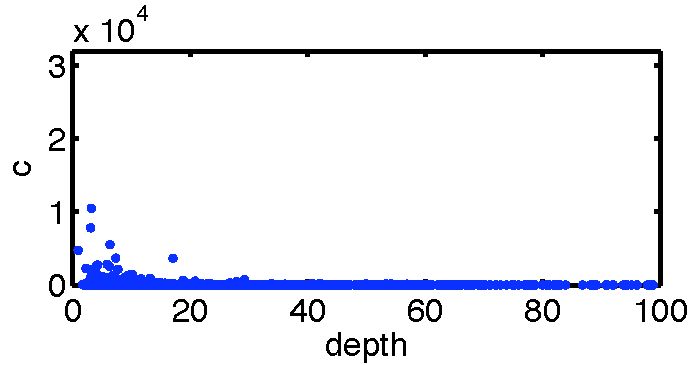
\includegraphics{figs/scatter_1024.pdf}} % [clip=true, viewport= 1in 1in 9in 9in]
%		\caption{Scatter plots to explore the relationship between the depth of a node and the total count}
%		\label{fig:restaurant_plots}
%	\end{center} 
%\end{figure*} 
